\chapter{HASIL YANG DIHARAPKAN}
\label{chap:hasilyangdiharapkan}

% Ubah bagian-bagian berikut dengan hasil yang diharapkan dari penelitian

\section{Hasil yang Diharapkan dari Penelitian}

Berdasarkan hasil pengujian yang telah dilakukan dalam tugas akhir ini, diharapkan penelitian ini menghasilkan suatu sistem deteksi kendaraan \emph{overdimension} dengan model yang di-\emph{deploy} di \emph{edge device} dengan akurasi dan kecepatan yang tinggi. Sistem ini diharapkan dapat digunakan pada gerbang tol untuk mendeteksi kendaraan \emph{overdimension} yang melintas.

% \begin{enumerate}
%   \item Membuat model deteksi kendaraan \emph{overdimension} yang dapat digunakan pada gerbang tol.
%   \item Membuat sistem deteksi kendaraan \emph{overdimension} yang dapat digunakan pada gerbang tol.
%   \item Membuat sistem deteksi kendaraan \emph{overdimension} yang dapat digunakan pada gerbang tol dengan akurasi yang tinggi.
%   \item Membuat sistem deteksi kendaraan \emph{overdimension} yang dapat digunakan pada gerbang tol dengan kecepatan deteksi yang tinggi.
% \end{enumerate}

\section{Hasil Pendahuluan}

Sampai saat ini, telah dilakukan studi literatur mengenai deteksi kendaraan \emph{overdimension} dan \emph{object detection}. Selain itu, telah dilakukan proses \emph{re-training} dari \emph{dataset} milik Ahmad Hamayan Nabih \parencite*{hamayan2024} dengan menggunakan model SSD MobileNetV2 di Jetson Nano. Hasil dari \emph{re-training} dapat dilihat pada \textbf{Gambar \ref{fig:retrain}}.

\begin{figure}[H]
    \centering
    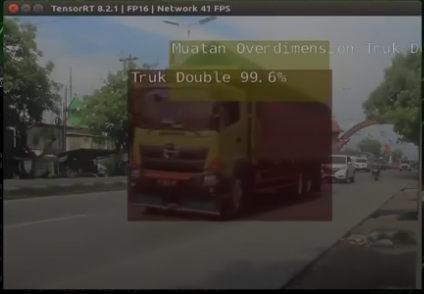
\includegraphics[scale=0.6]{gambar/bab4-hasil-retrain.png}
    \caption{Hasil \emph{re-training} \emph{dataset} dengan SSD MobileNetV2}
    \label{fig:retrain}
\end{figure}

Dari hasil di atas, dapat dilihat bahwa model yang dihasilkan sudah mampu mendeteksi kendaraan \emph{overdimension} dengan cukup baik dan stabil di 35 - 40 FPS.